% CVPR 2022 Paper Template
% based on the CVPR template provided by Ming-Ming Cheng (https://github.com/MCG-NKU/CVPR_Template)
% modified and extended by Stefan Roth (stefan.roth@NOSPAMtu-darmstadt.de)

\documentclass[10pt,twocolumn,letterpaper]{article}

%%%%%%%%% PAPER TYPE  - PLEASE UPDATE FOR FINAL VERSION
%\usepackage[review]{cvpr}      % To produce the REVIEW version
\usepackage{cvpr}              % To produce the CAMERA-READY version
%\usepackage[pagenumbers]{cvpr} % To force page numbers, e.g. for an arXiv version

% Include other packages here, before hyperref.
\usepackage{graphicx}
\usepackage{amsmath}
\usepackage{amssymb}
\usepackage{booktabs}


% It is strongly recommended to use hyperref, especially for the review version.
% hyperref with option pagebackref eases the reviewers' job.
% Please disable hyperref *only* if you encounter grave issues, e.g. with the
% file validation for the camera-ready version.
%
% If you comment hyperref and then uncomment it, you should delete
% ReviewTempalte.aux before re-running LaTeX.
% (Or just hit 'q' on the first LaTeX run, let it finish, and you
%  should be clear).
\usepackage[pagebackref,breaklinks,colorlinks]{hyperref}


% Support for easy cross-referencing
\usepackage[capitalize]{cleveref}
\crefname{section}{Sec.}{Secs.}
\Crefname{section}{Section}{Sections}
\Crefname{table}{Table}{Tables}
\crefname{table}{Tab.}{Tabs.}


%%%%%%%%% PAPER ID  - PLEASE UPDATE
\def\cvprPaperID{******} % *** Enter the CVPR Paper ID here
\def\confName{CVPR}
\def\confYear{2022}


\begin{document}

%%%%%%%%% TITLE - PLEASE UPDATE
\title{Compare Study of traditional machine learning and deep learning algorithm in Face Recognition}

\author{Lujie Ma\\
School of Computer Science\\
University of Adelaide\\
{\tt\small a1810558@adelaide.edu.au}
% For a paper whose authors are all at the same institution,
% omit the following lines up until the closing ``}''.
% Additional authors and addresses can be added with ``\and'',
% just like the second author.
% To save space, use either the email address or home page, not both
}
\maketitle

%%%%%%%%% ABSTRACT
\begin{abstract}

 Identifying objects in the image is now popular in our daily life. Image recognition refers to the task of inputting an image into a neural network and 
 having it output label for that image. A subset of image classification is object detection, where specific instances of objects are identified as belonging 
 to a certain class like animals, cars, or people. This paper will focus on face recognition.
\end{abstract}


%%%%%%%%% Part 1: introduction
%------------------------------------------------------------------------
\section{Introduction}
\label{sec:intro}

Face recognition is very common in our daily life, identification is relying on face recognition.
Such as tracking student or worker attendance; unlock the phone; law enforcement; airports and border control; finding missing persons and so on.
Under the influence of the new crown epidemic (COVID-2019),
there is no requirement to get in physical contact with the face recognition, which helps in controlling the spread of diseases like viruses.
By the way, face recognition does not disturb the privacy of the individual.
Over the past decades, extensive research has made great progress in face recognition. 
Deep learning and traditional machine learning algorithm is widely used in this area (face recognition). 
We will Discuss the difference between apply the traditional machine learning algorithm and deep learning in face recognition.


%---- figure part -------
\begin{figure}[htp]
  \centering
  %\fbox{\rule{0pt}{2in} \rule{0.9\linewidth}{0pt}}
   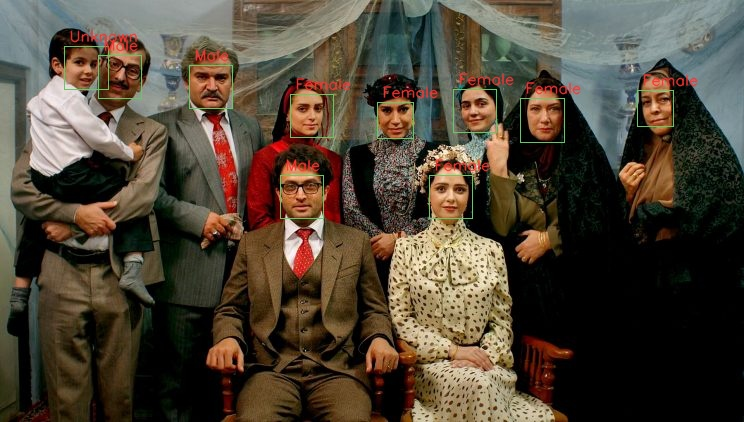
\includegraphics[width=0.9\linewidth]{image.jpeg}

   \caption{Example of the output of face recognition. Identify the gender of a person through face recognition by using . ~\cite{github}}
\end{figure}




%%%%%%%%% Part 2: introduction
%------------------------------------------------------------------------
\section{Steps of Face Recognition}
\label{steps info}

Facial recognition is a technology that can recognise a person only by looking at them.
The steps of face recognition is include preparing the dataset, pre-processing, feature extraction and face verification. 



%-------------------------------------------------------------------------
\subsection{preparing the dataset}
We can get images of faces in the equipment. e.g. cameras, phones.
Or, we can get the data sets online by downloading them.
There must be included the face in the images. 

%-------------------------------------------------------------------------
\subsection{Pre-processing}
Face Alignment is also a step of pre-processing the data sets.
Faces in the original data sets can not be used directly, we should do the pre-processing to the data sets.
The purpose of using pre-processing steps in face detection system is to speed up the detection process and reducing false positives.
We should extract the images which is wrong. e.g. exclude the image which do not have human faces.


There has some methods in the pre-processing part.
One of methods is based on linear image transform (LIT) which ignores scanning a number of non-face windows. 
The second one utilizes regional minima (RM) to reject non-face windows. ~\cite{NAFCHI2012162}


%-------------------------------------------------------------------------
\subsection{Feature Point Extraction}
Feature extraction is important which will greatly affect the accuracy in the final part (face verification).
This part entails measuring and extracting numerous characteristics from the faces.
We could use machine learning algorithm or deep learning to help us to get a better strategy to extract the features in faces.


%-------------------------------------------------------------------------
\subsection{Face Verification}
The final step is face verification. This is the most complex step during the face recognition.
By extracting the feature points in the previous step, we need to compare against the database features.
If there is a match, return the face is recognised successfully; if not, return the faces is not included in the database.
We can use some match strategy to increase the accuracy in this part. e.g. top-k strategy.



%%%%%%%%% Part 3: Traditional Machine Learning algorithm
%------------------------------------------------------------------------
\section{Traditional Machine Learning Algorithm}
\label{Traditional Machine Learning algorithm}

There are many algorithms in traditional machine learning, popular machine learning algorithms include: Linear Regression, Logistic Regression, SVMs, K-
Nearest Neighbour, Decision Trees, Random Forests, PCA, K-Means Clustering, and Gradient-boosting trees. 
Some algorithm's output is interpretable, e.g. logistic regression, decision tree. This is one of benefits of traditional machine learning.


%-------------------------------------------------------------------------
\subsection{K-Nearest Neighbour algorithm} There is the formula of K-Nearest Neighbour algorithm:
\begin{equation}
  d(p,q) = d(q,p) = \sqrt{\sum_{i=1}^{n} (q_i - p_i)^{2}}
 \end{equation}
 
KNN is the most practical / non –parametric approach for facial recognition. ~\cite{knn}
based on features such as eyes, nose, eyebrows, mouth, ears within the source image. 
It achieves its robustness by normalising the size and orientation of face. ~\cite{4}

The disadvantages of KNN: 
Time complexity for each prediction is O(MNlog(k)) where M is the dimension of the data, N is the size or the number of instances in the training data.
Therefor, KNN method not work good in a large datasets.



%%%%%%%%% Part 4: Deep Learning Algorithm
%------------------------------------------------------------------------
\section{Deep Learning Algorithm}
In recent year, deep learning have been recommended to solve the problems in computer vision area.
The benefit of deep learning is that deep learning is able to perform automatic feature extraction from the data.

%---- figure part CNN -------
\begin{figure}[htb]
  \centering
  %\fbox{\rule{0pt}{2in} \rule{0.9\linewidth}{0pt}}
   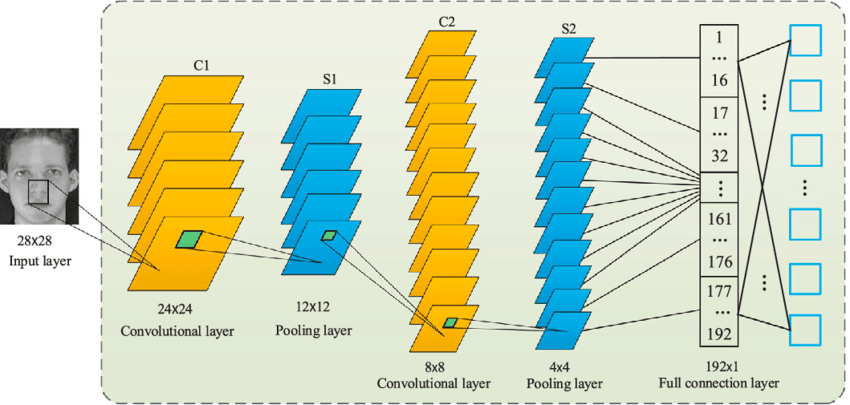
\includegraphics[width=0.9\linewidth]{CNN.png}

   \caption{CNN model ~\cite{cnn}}
\end{figure}


%-------------------------------------------------------------------------
\subsection{Convolutional Neural Networks}



%%%%%%%%% Part 5: Conclusion
%------------------------------------------------------------------------
\section{Conclusion}






%%%%%%%%% REFERENCES
{\small
\bibliographystyle{ieee_fullname}
\bibliography{egbib}
}

\end{document}
